\documentclass[twocolumn,a4j]{jarticle}
\usepackage{graphicx, color, hyoshi, epsbox}
%\usepackage{float}
\usepackage{color,fancyhdr}
\usepackage{multirow}
\renewcommand{\figurename}{Fig.}
\renewcommand{\tablename}{Table}
\newcommand{\ve}[1]{\mbox{\boldmath $#1$}}
%Fig.やTableを太字にし,キャプションのコロンを消す
%--ここから--
\makeatletter
\long\def\@makecaption#1#2{%
\vskip\abovecaptionskip
\iftdir\sbox\@tempboxa{#1\hskip1zw#2}%
\else\sbox\@tempboxa{\textbf{#1} #2}%
\fi
\ifdim \wd\@tempboxa >\hsize
\iftdir #1\hskip1zw#2\relax\par
\else \textbf{#1} #2\relax\par\fi
\else
\global \@minipagefalse
\hbox to\hsize{\hfil\box\@tempboxa\hfil}%
\fi
\vskip\belowcaptionskip}
\makeatother
%--ここまで--

%
%
% /* Header & Footer */
%
\pagestyle{fancy}
\rhead{\thepage}
\renewcommand{\theenumi}{\alph{enumi}}
%\cfoot{\footnotesize{大阪大学大学院基礎工学研究科機能創成専攻機能デザイン領域}}
\cfoot{}
%

\newcommand{\namelistlabel}[1]{\mbox{#1}\hfil}
 \newenvironment{namelist}[1]{%
 \begin{list}{}
  {\let\makelabel\namelistlabel
   \settowidth{\labelwidth}{#1}
   \setlength{\leftmargin}{1.1\labelwidth}}
  }{%
 \end{list}}
%
\def\inttt{\int\!\!\!\!\int\!\!\!\!\int}
\def\intt{\int\!\!\!\!\int}
\def\d{\partial}
\def\tab{\qquad\qqua d}
\def\bold#1{\mbox{\boldmath$#1$}}
\def\ebold#1{\mbox{\boldmath$#1$}_e}
%
\begin{document}
%%%%%%表紙%%%%%%%
\begin{titlepage}
\baselineskip=24pt
%\vspace*{30mm}
\vspace*{10mm}
\hspace*{10mm}
\begin{center}
{{\LARGE \underline{特別研究}}}
\vspace*{10mm}\\
{\LARGE 導電性布,シリコンを用いた柔軟性を持つ伸縮センサ}
%\hspace{-1em}
\end{center}
\vspace*{40mm}

%
%\hspace*{50mm}
%{\Large
%\begin{flushright}
\begin{center}
{\large 令和 2 年 2 月 17 日 提出}\\
\end{center}

\hspace*{40mm}
{\Large
\begin{center}
$
\left.
\begin{array}{l}
\mbox{西川 敦 教授}\\
\mbox{平井 宏明 准教授}\\
\mbox{松居 和寛 助教}\\
\end{array}
\right \}
$指導\\
\end{center}
}

\vspace*{20mm}
\begin{center}
{\Large
\hspace*{-2em}
大阪大学 基礎工学部 システム科学科 機械科学コース

09C16114 丹羽 英人
\hspace*{-1em}\\
\hspace*{-2em}

\hspace*{-1em}}
\vspace*{0mm}
\end{center}
\end{titlepage}
\markright{\hfill}
\pagenumbering{roman}

\baselineskip=18pt

\baselineskip=16pt
\clearpage
\pagenumbering{arabic}
%%%%%%%%%%%%%%%%%%%%%%%%%%%%%%%%%%%%%%%%%%%%%%%%%%%%%%%%%%%%%%%%%%%%%
\section{研究背景}
%TODO:伸縮センサのお話を書く
soft robotics toolkit\cite{MITSoftRobot}において,シリコンと導電性布をもちいた伸縮センサが紹介されていた.本センサは,伸縮性に優れており,柔軟性も兼ね備えたものとなっている.また,製作コストも\$23と非常に安価なものであると紹介されている.
\begin{figure}[h]
    \begin{center}
        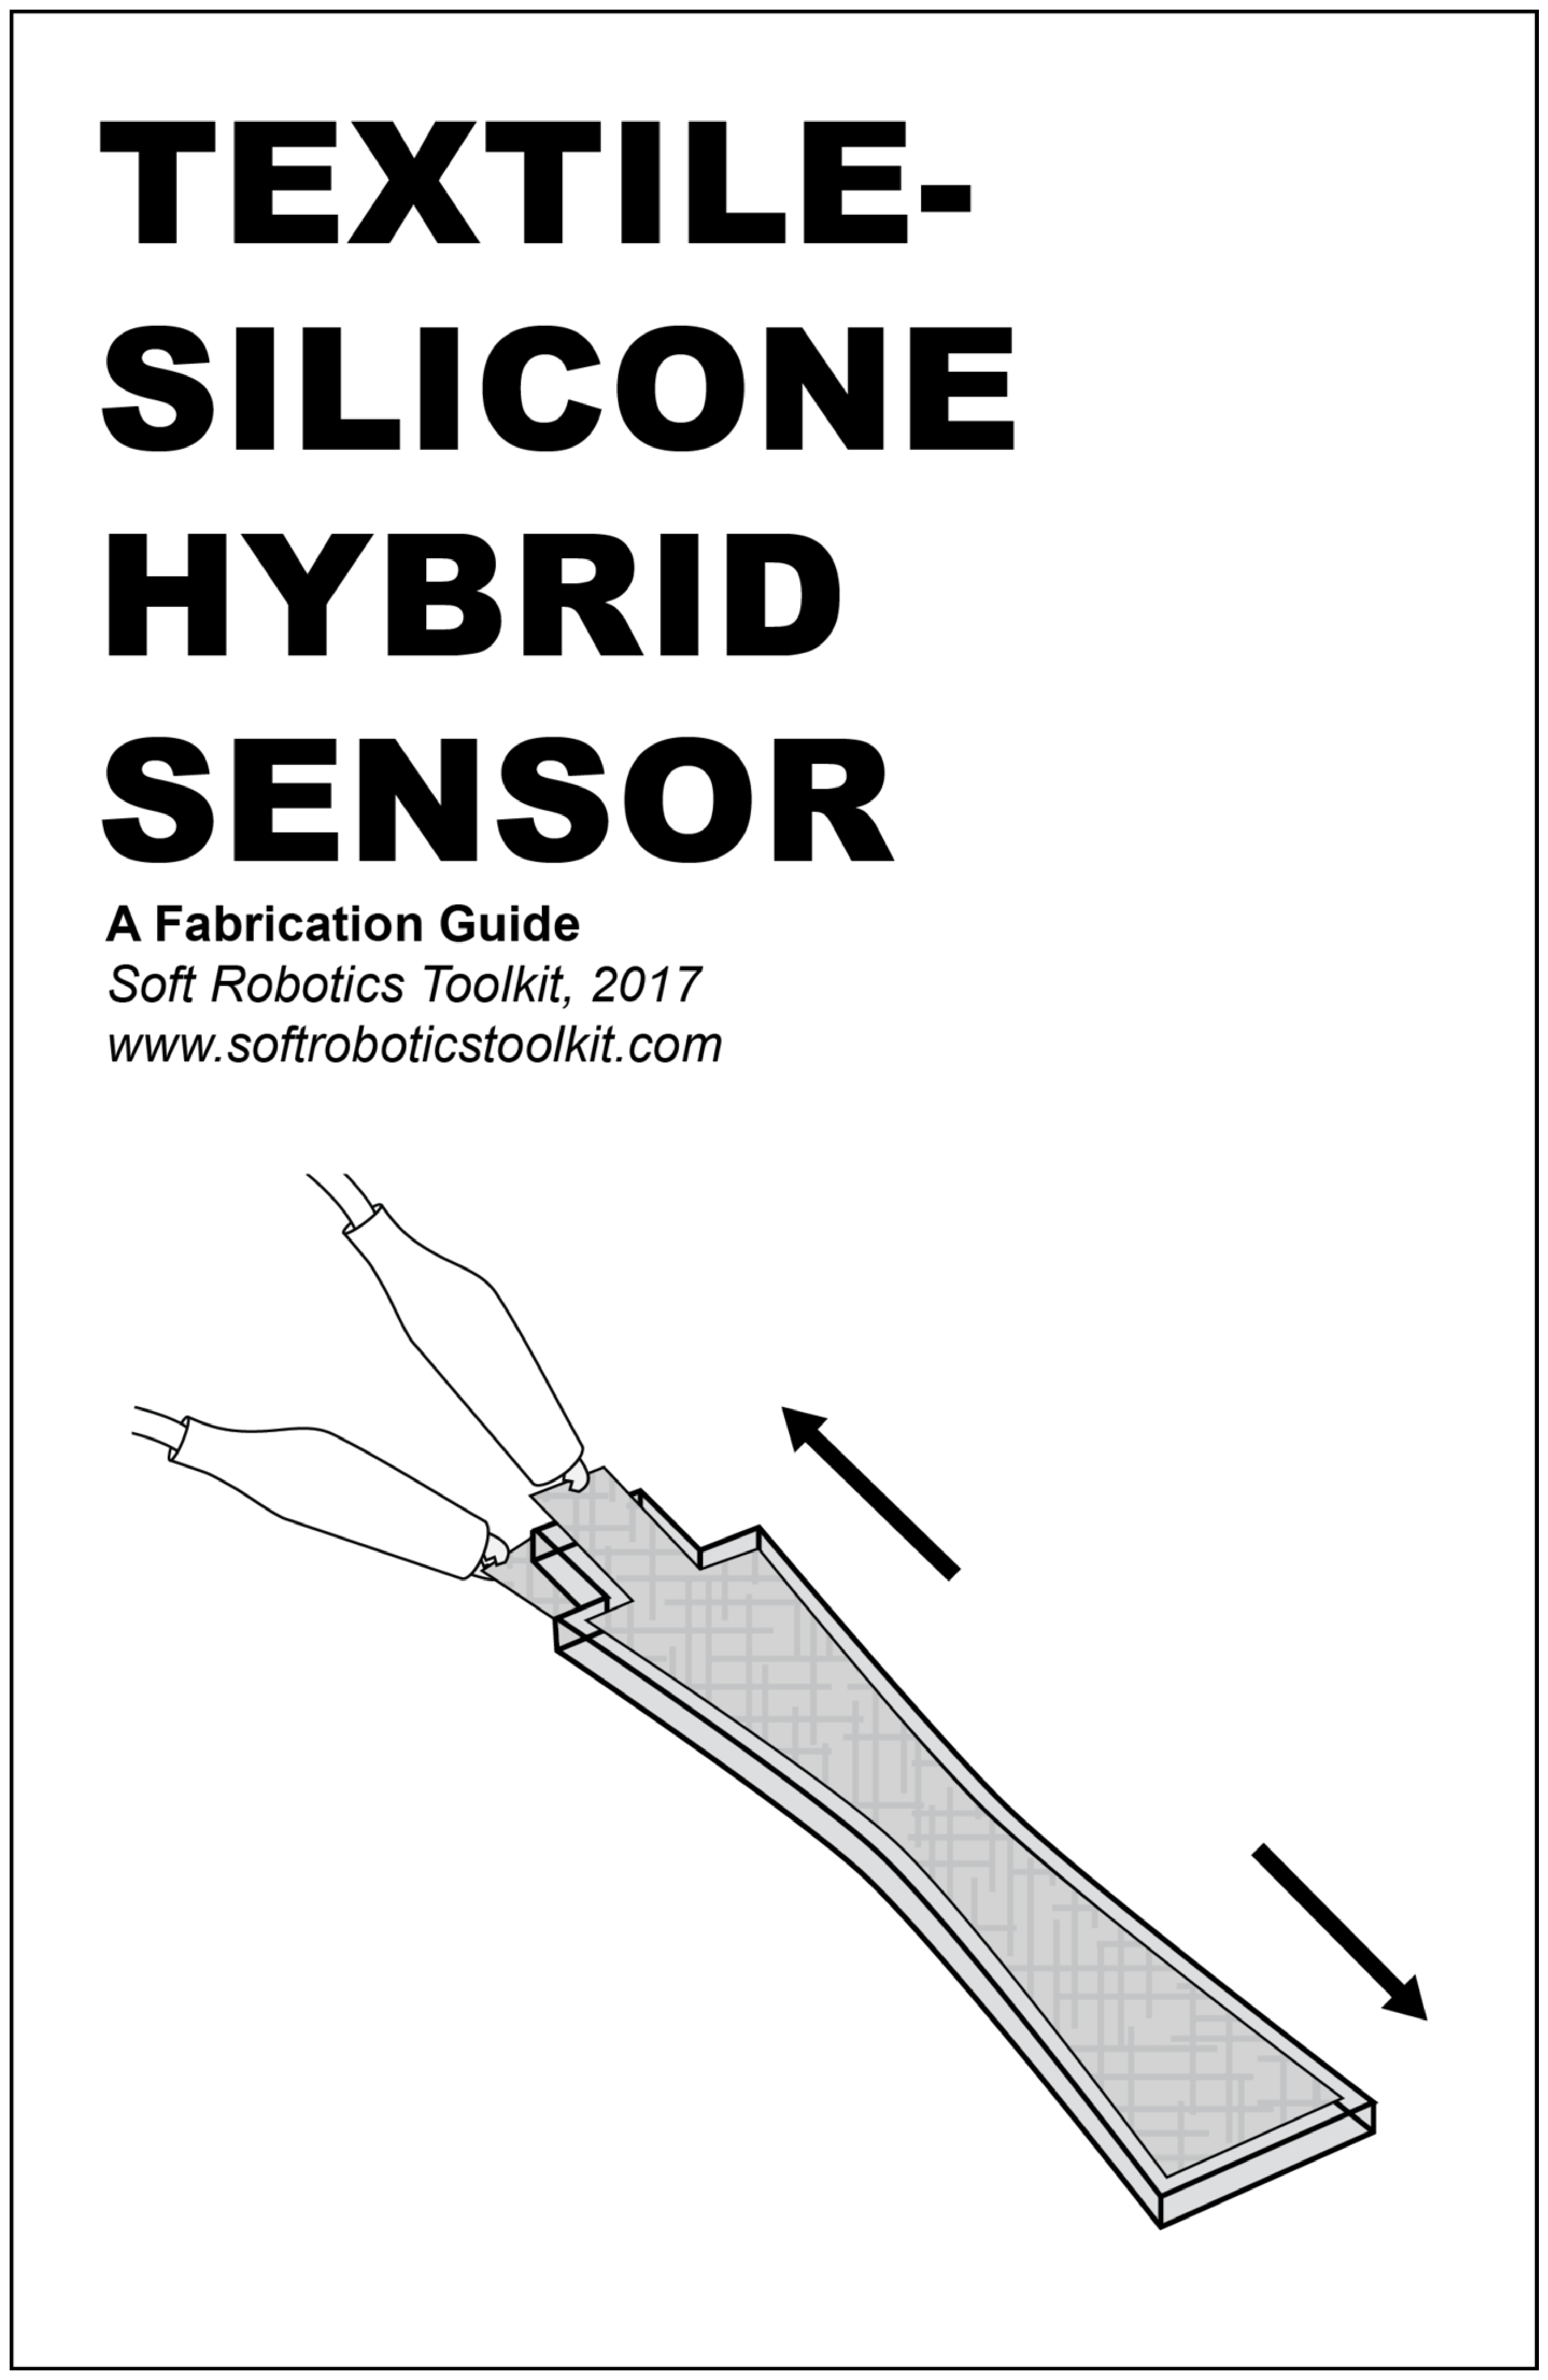
\includegraphics[width=0.5\columnwidth,clip]{Photo/BackGround/MITSoftRobotics.eps}
        \caption{soft roboticstool kit 表紙\cite{MITSoftRobot}}
        \label{MITSoftRobot表紙}
    \end{center}
\end{figure}

%TODO:初号機体のお話を書く
%TODO:初号機関連の研究のリファレンスを貼る
当研究室において先行研究として,人間の筋肉を模した空気圧人工筋をもちいたペダリングロボット(初号機)が存在する.これは,人間のペダリング動作における筋シナジーの計測を行い,ロボットに再現させるものであった.筋シナジーの計測は片麻痺患者,健常者ともに行い,片麻痺患者におけるペダリング動作時の特徴的な活動状態を健常者との比較を行った.本ロボットは,腰がサドル上に固定された状態で股関節,膝関節,足首関節それぞれがピッチ方向にのみ自由度を持っており2次元平面上における動作を再現することが出来た.また本動作を再現するために空気圧人工筋を片足8筋分用いて行っていた.
\begin{figure}[h]
 \begin{center}
  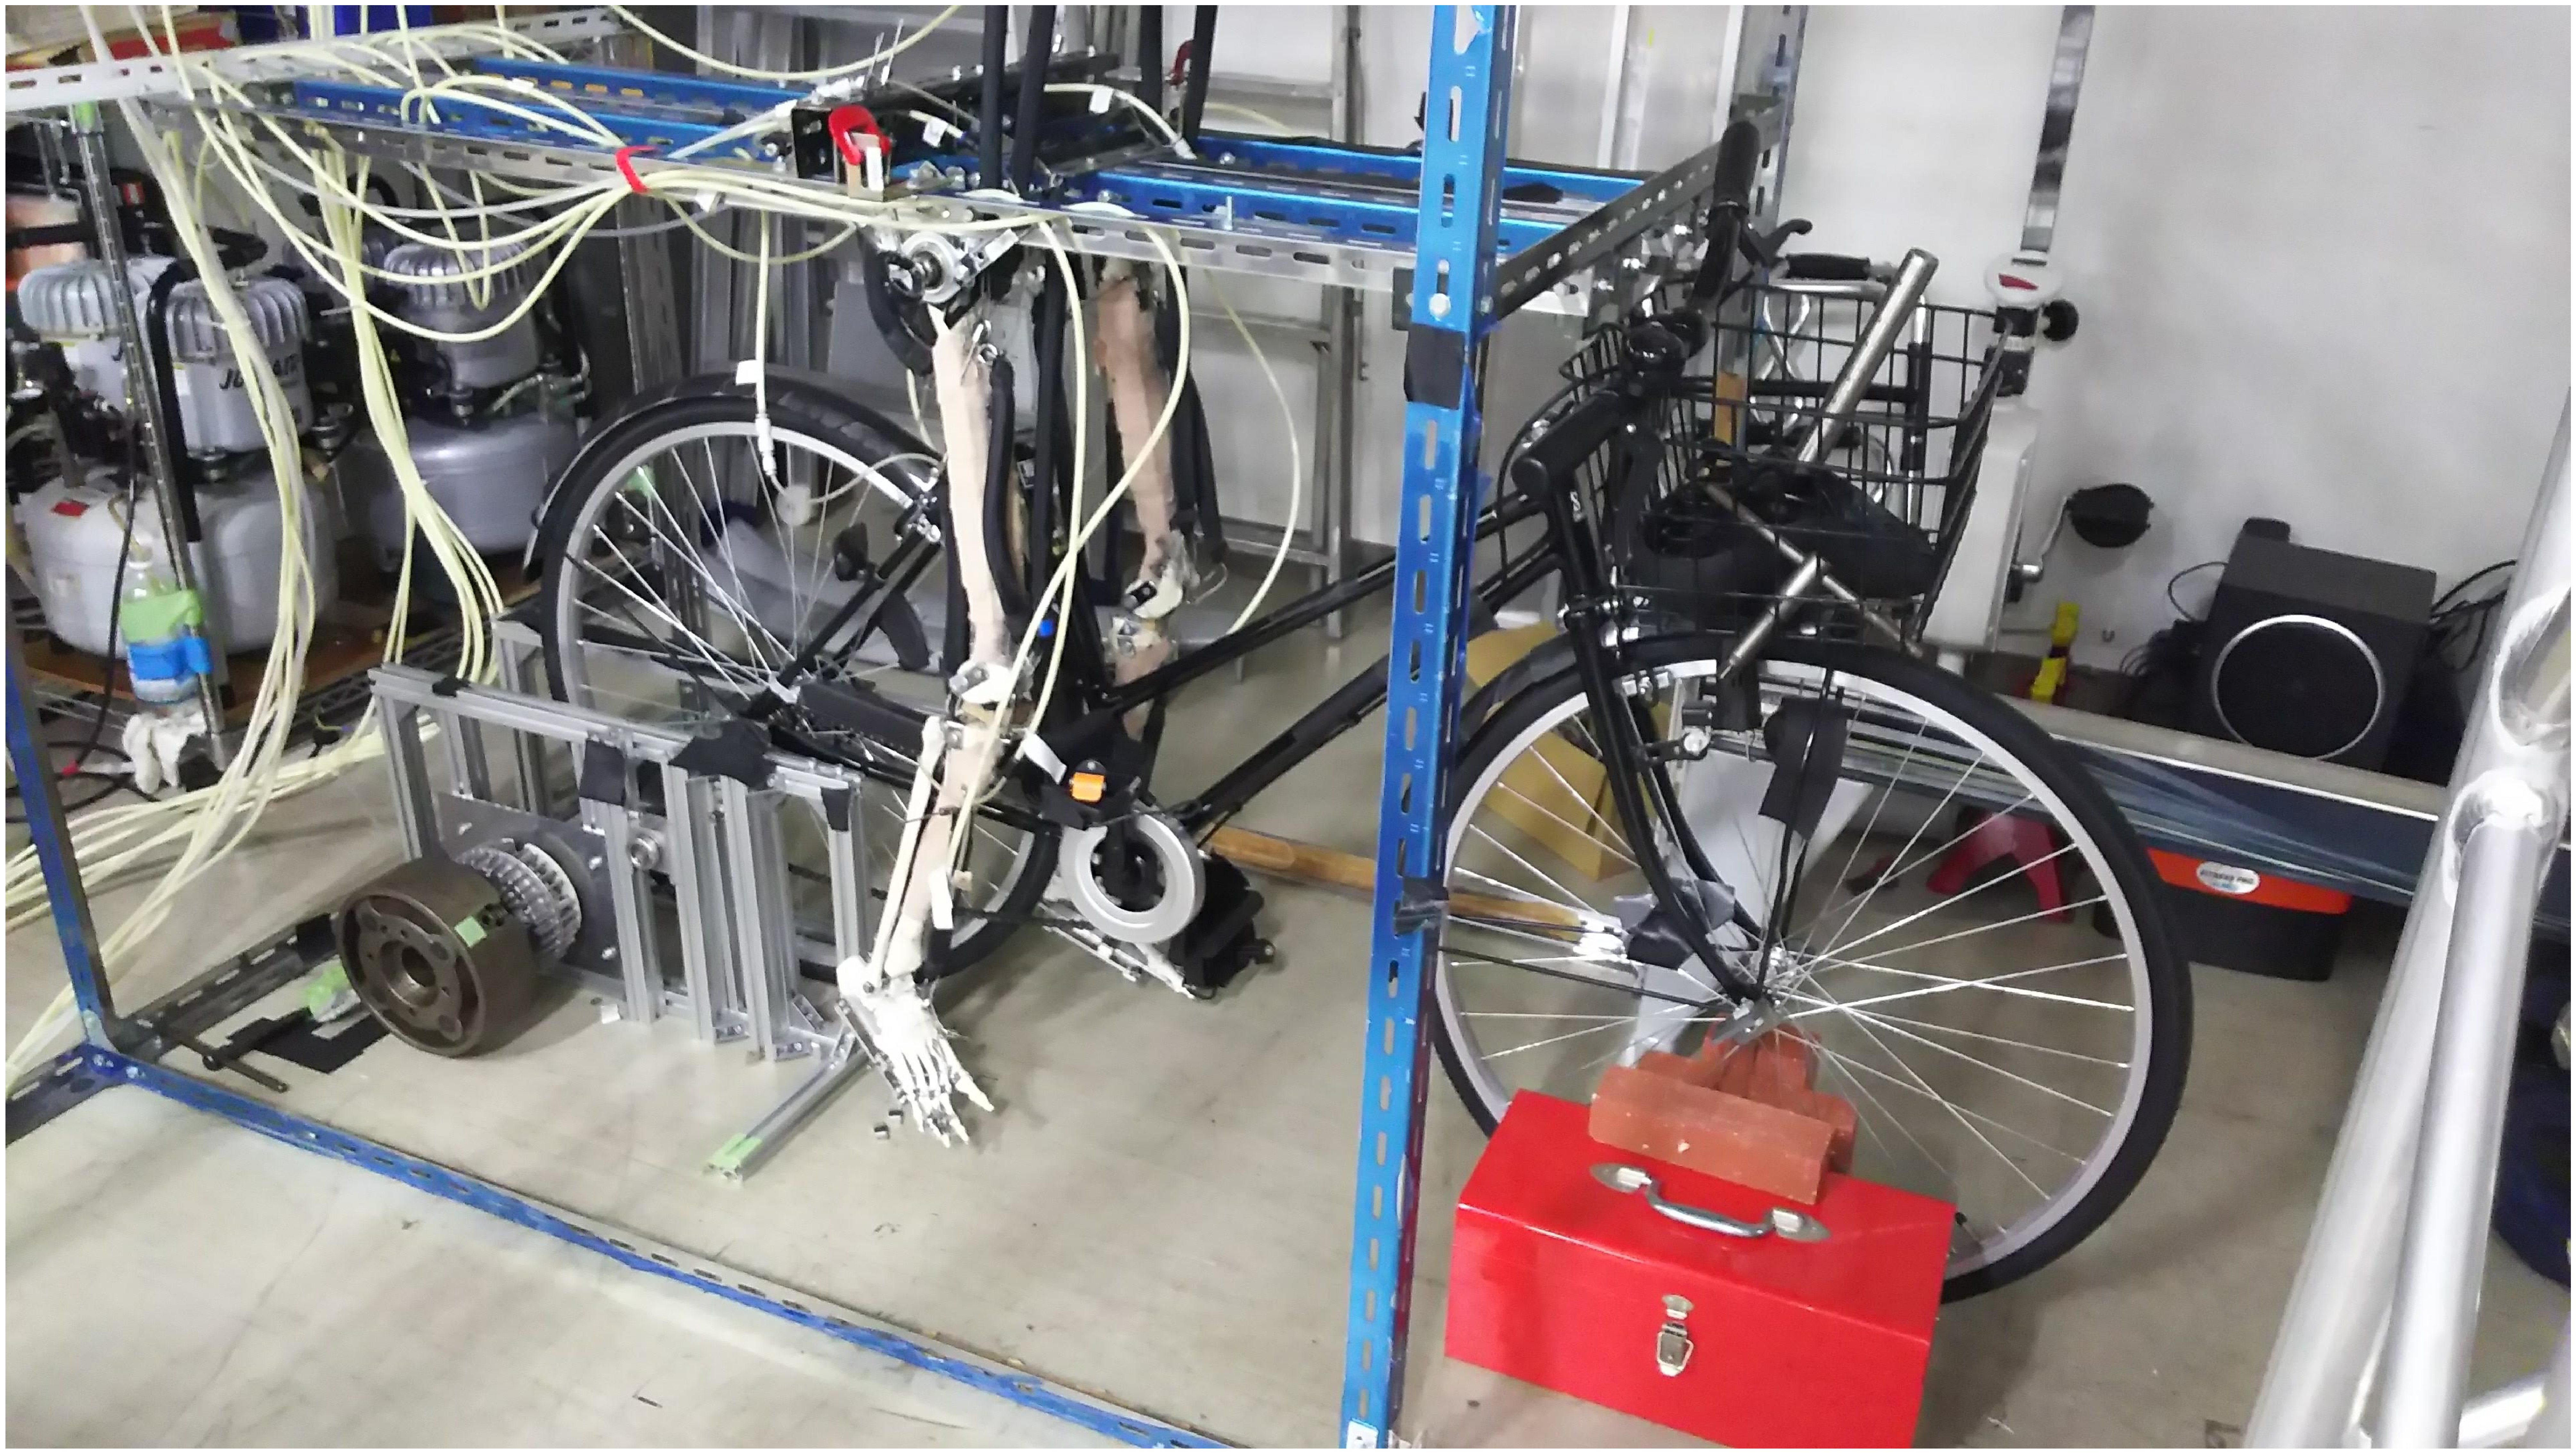
\includegraphics[width=0.75\columnwidth,clip]{Photo/BackGround/1st.eps}
  \caption{ペダリングロボット(初号機)}
  \label{初号機}
  \end{center}
\end{figure}

%TODO:2号機のお話を書く
%TODO:2号機関連の研究のリファレンスを貼る
また,先述の初号機を元にして腰を固定していない状態の二足歩行型ロボット(2号機)も製作された.こちらは先述のロボットと異なり腰が固定されておらず,二足歩行可能な形となっている.一方で関節動作に関しては先述のロボットと同様の形となっており,股関節,膝関節,足首関節それぞれがピッチ方向にのみ自由度を持っており2次元平面上における動作を再現することが出来た.先述のロボットと同様に,筋シナジーベクトルを利用し片麻痺患者と健常者の歩行の比較をロボット上で行った.
\begin{figure}[h]
  \begin{center}
  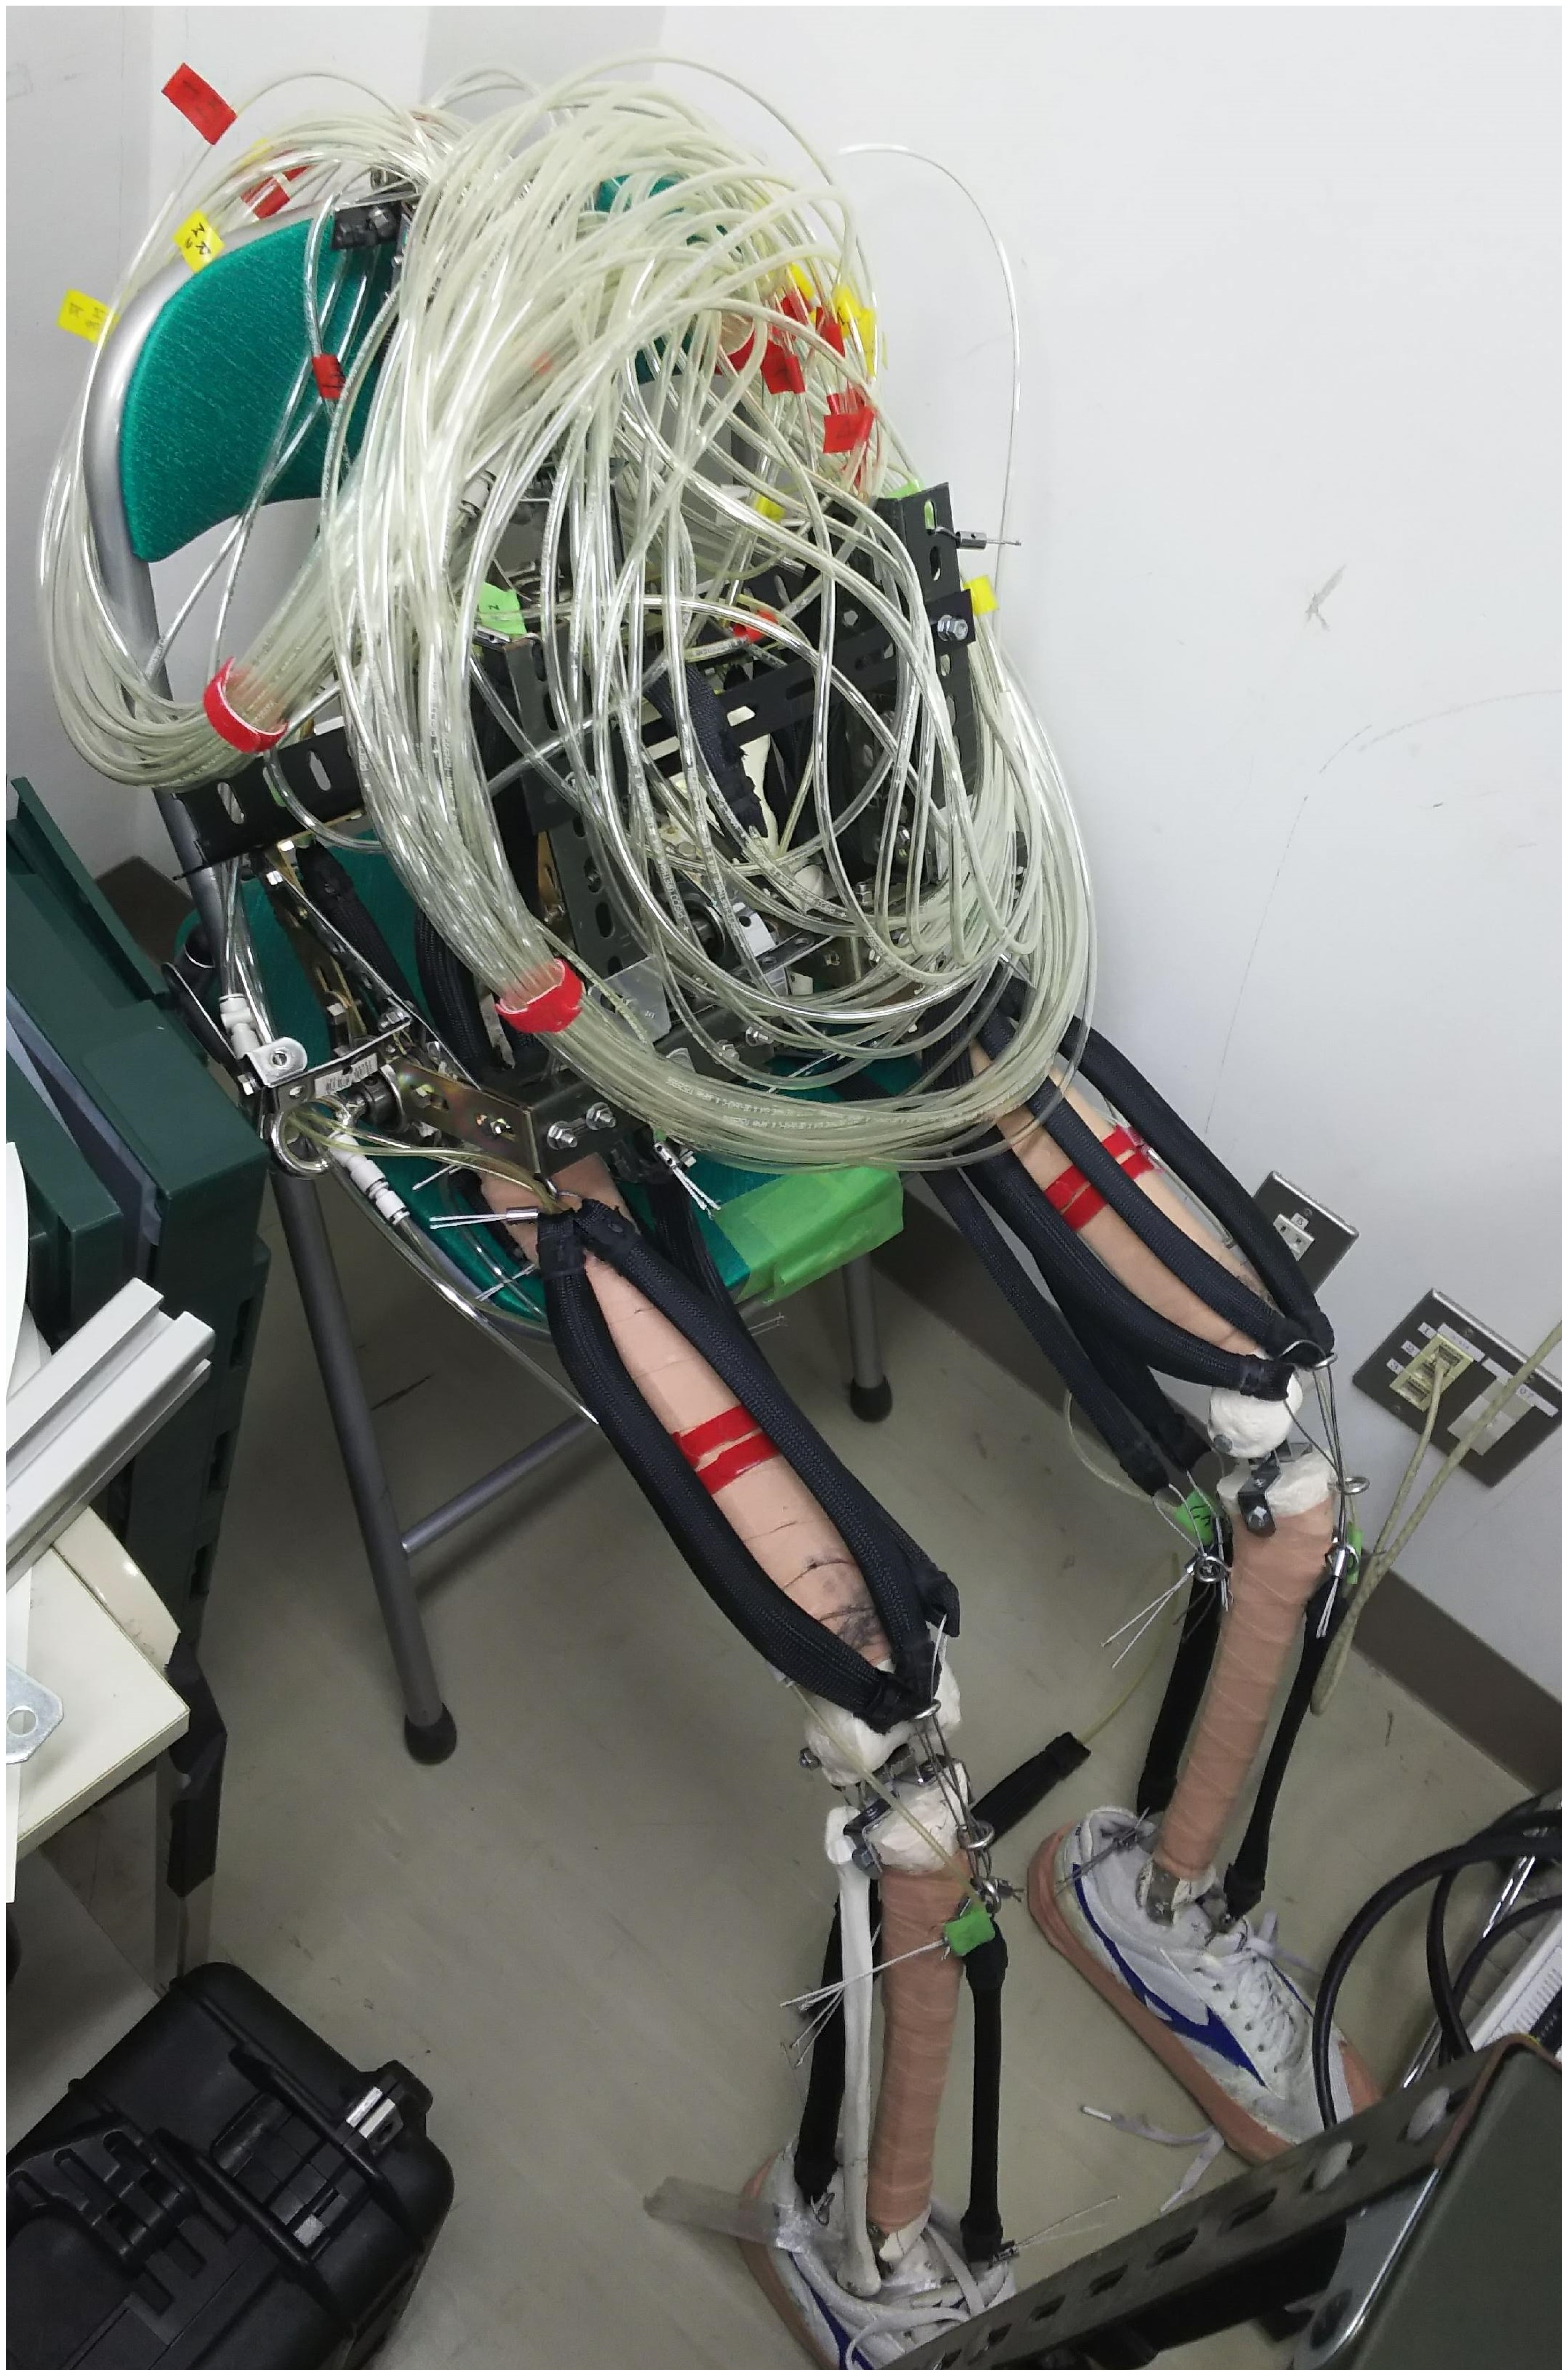
\includegraphics[width=0.5\columnwidth,clip]{Photo/BackGround/2nd.eps}
  \caption{二足歩行ロボット(2号機)}
  \label{2号機}
 \end{center}
\end{figure}

%TODO:3号機のお話を書く
これら,ペダリングロボット(初号機),2足歩行ロボット(2号機)の経験を踏まえ,今回新たに2足歩行ロボット(3号機)の開発を行った.従来の2足歩行ロボットでは自由度の制約が大きく,2次元平面上のみでの動作となっていたものが3次元空間上で動かせるものとした.

股関節部分の自由度

足関節の自由度が従来の2足歩行ロボット(2号機)ではピッチ方向の1自由度であった。一方で実際の人間の自由度はこれに加えてロール方向,ヨー方向も存在し3自由度である.

%TODO:これらを統合し,筋肉の伸長を巻き込んだシステムの話をする
今回開発を行った導電性布,シリコンを用いた伸縮センサを空気圧人工筋に組み合わせ

\section{動作モデル}
\subsection{足首}
%TODO:足首周りの動作関係のお話をする
%付着筋肉のお話もする
付着筋肉 %何の筋肉をもちいた?

ボールジョイントを用いて,ロール・ピッチ・ヨー各軸に自由度を持たせた.

\subsection{伸縮センサ}
%TODO: 大学PCで書いた伸縮センサCADのレンダリング画像を挿入する
伸縮センサはFig.\ref{伸縮センサ断面図}において示す通り,柔軟で弾性変形する伸縮性シリコン(絶縁層)と導電性布電極(導電層)の重ね合わせによって構成されている.これは,誘電体をシリコン,極板を導電性布としたコンデンサとなっている.

\begin{figure}[h]
    \begin{center}
        \label{伸縮センサ全体図}
        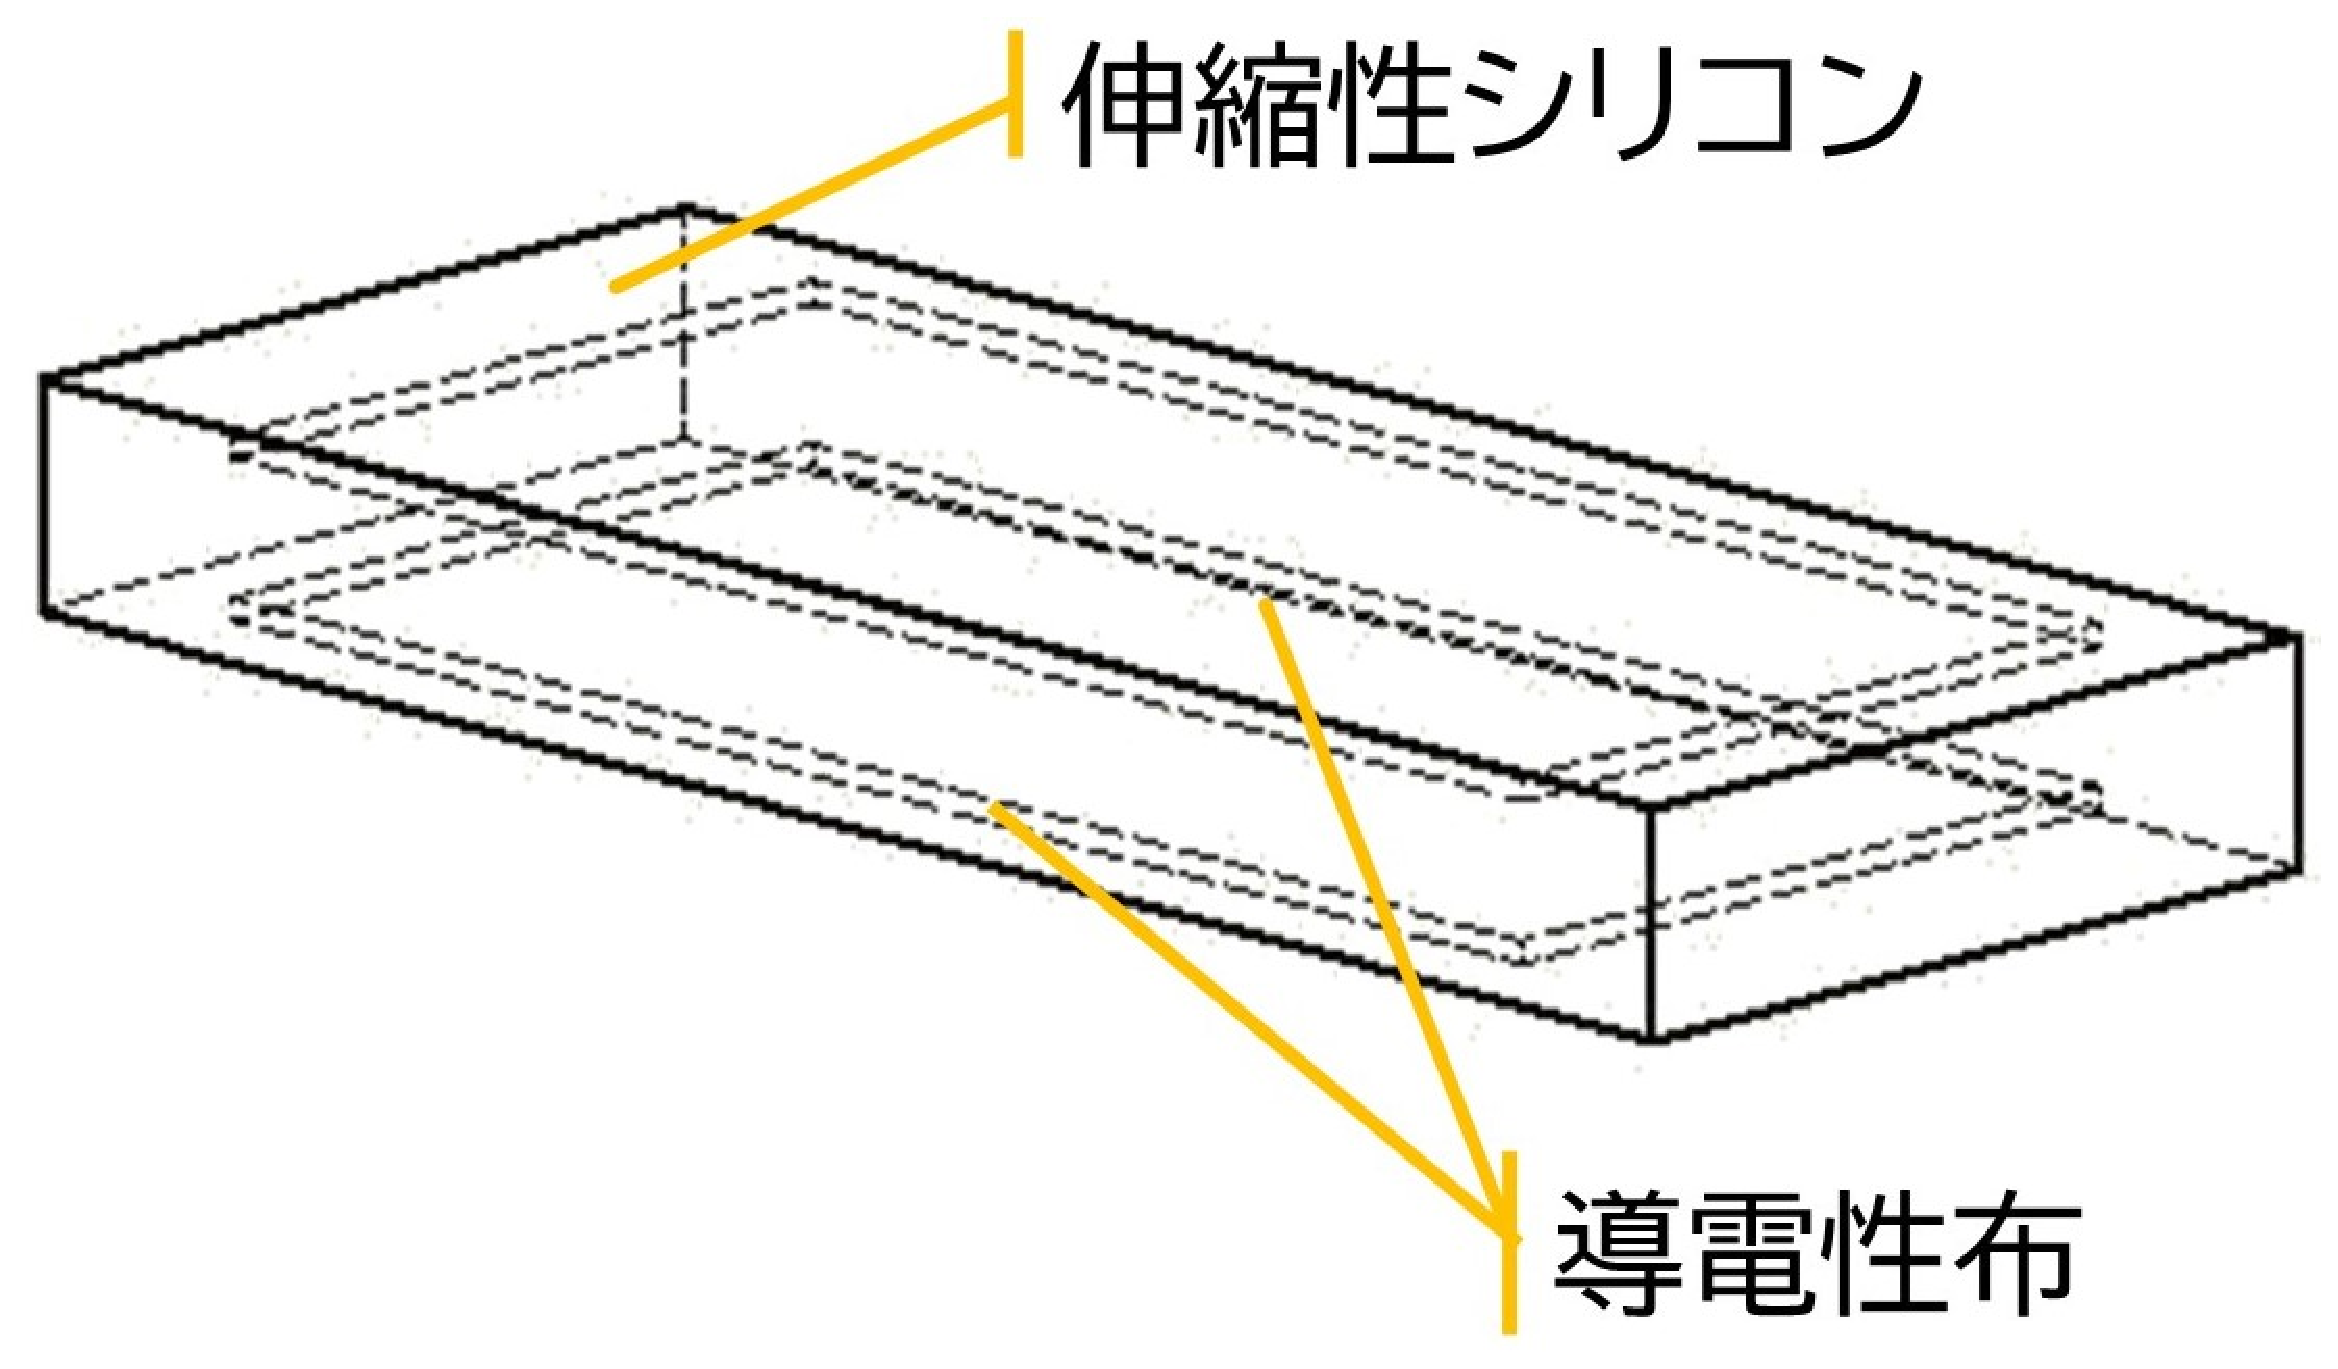
\includegraphics[width=0.85\columnwidth,clip]{Photo/BackGround/画像_説明付き/スライド1.eps}
        \caption{伸縮センサ全体図}
    \end{center}
\end{figure}
\begin{figure}[h]
    \begin{center}       
        \label{伸縮センサ断面図}
        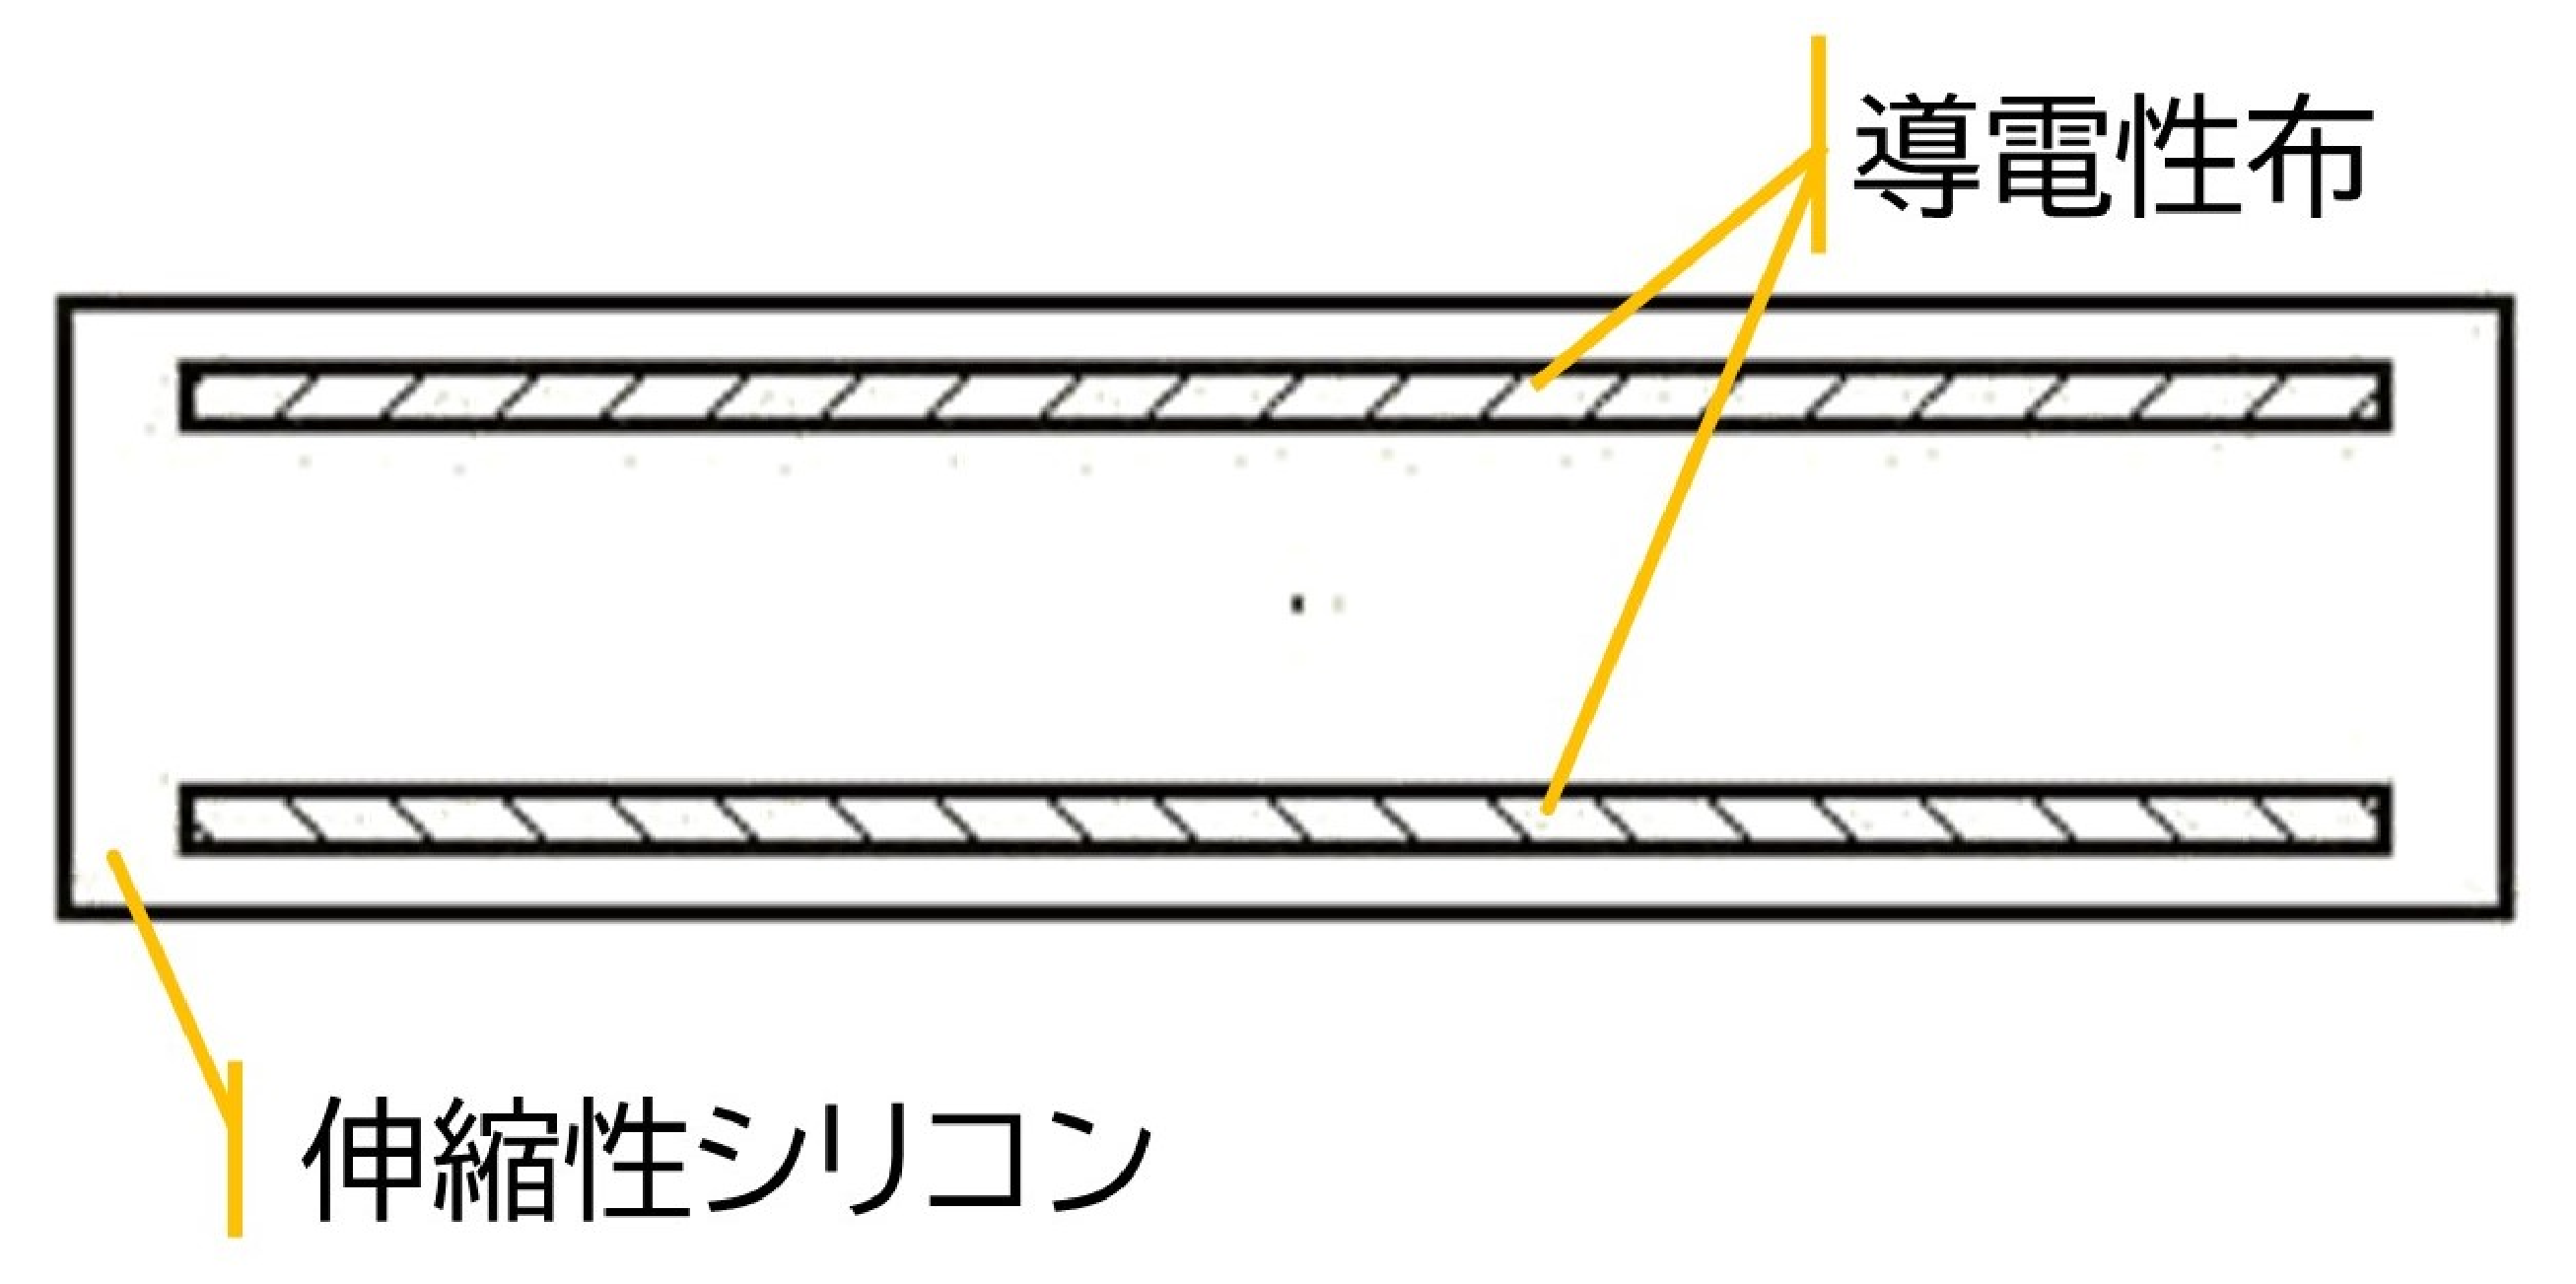
\includegraphics[width=0.85\columnwidth,clip]{Photo/BackGround/画像_説明付き/スライド2.eps}
        \caption{伸縮センサ断面図}
    \end{center}
\end{figure}

ここで伸縮センサ中の導電性布の表面積$S$,誘電体の厚さを$d$,真空の誘電率を$\epsilon{}_0$,シリコンの比誘電率を$\epsilon{}_s$とすると,
\begin{eqnarray}
    C=\epsilon{}_0\epsilon{}_s\frac{S}{d}
\end{eqnarray}
といった式となる.ここで体積が一定の変化であると仮定すると, 

ここで静電容量の変化を$\Delta{}C$,厚みの変化を$\Delta{}d$とそれぞれすると、

一方で,伸縮センサは引張方向のみに応力がかかる単軸応力状態であると見れるため,引張方向のひずみ$\gamma$,引張方向の垂直応力$\sigma$,ヤング率$E$とそれぞれすると,
\begin{eqnarray}
    \sigma=E\gamma
    \label{フックの法則}
\end{eqnarray}
といった式がフックの法則により示される.また,引張方向に対して直交方向である垂直ひずみ$\gamma{}_s$,ポアソン比$\mu$とすると,
\begin{eqnarray}
    \mu = \frac{\gamma{}_s}{\gamma}
    \label{ポアソン比}
\end{eqnarray}
といった式となる.

\subsection{伸縮センサ計測回路}
%TODO:伸縮センサ計測回路に関しての記述を行う
%TODO:RC回路の電圧を掛けたときの時定数の様子をオシロスコープで撮影した画像が欲しい
伸縮センサは静電容量の変化で伸縮状況を示す.故に今回は静電容量の変化を計測することができるシステムを用いればよい.そのため,NucleoF303K8にRC回路を用いて可変静電容量に関して,固定抵抗器を用いて計測を行った.

\begin{figure}[h]
 \begin{center}
    %Voutの向きを出力にする
  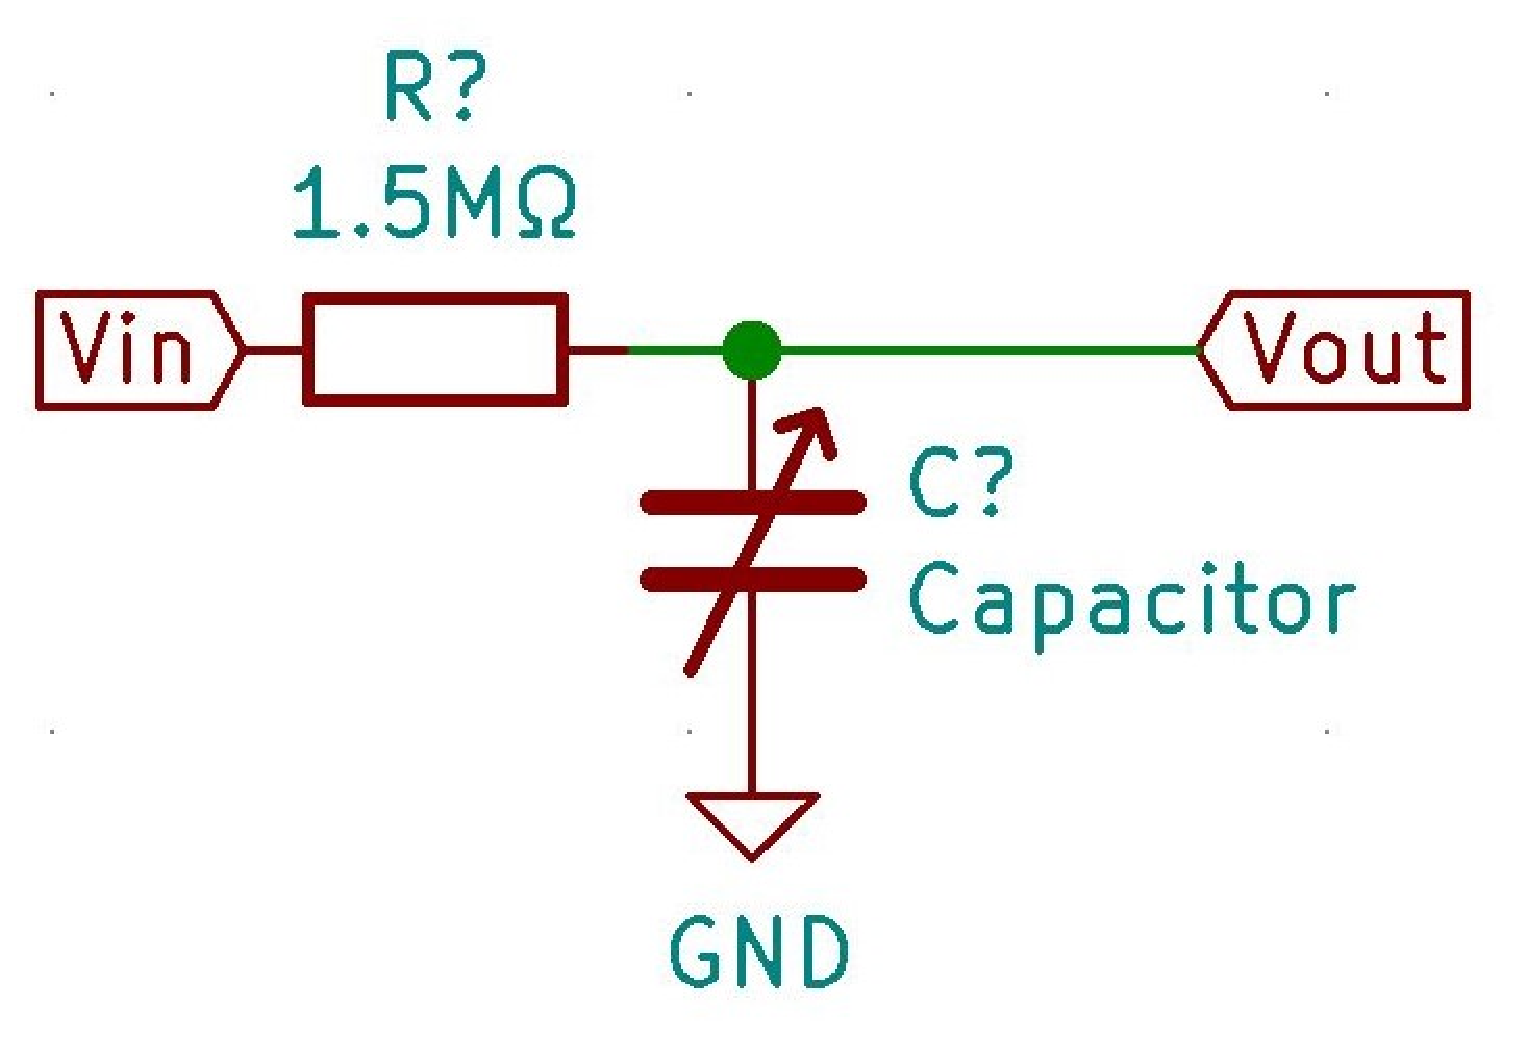
\includegraphics[width=0.75\columnwidth,clip]{Photo/BackGround/RC.eps}
  \caption{RC回路}
  \label{RC}
 \end{center}
\end{figure}

これらの計測に関して,1つのマイコンを用いて複数の伸縮センサの計測を行うと計測周期が低下し,計測精度の低下が懸念された.これを踏まえ,1つのマイコンで計測を行う伸縮センサの数を2個とした.一方で今回,足首を中心とした筋の伸縮の計測を行うため6チャンネル分の計測を行う必要がある.故に,マイコン3枚分の計測システムを用意した.これらをCAN通信(Controller Area Network)と同期信号を用いて計測のデータ取得,同期を行った.
\begin{figure}[h]
 \begin{center}
  
\includegraphics[width=0.75\columnwidth,clip]{Photo/BackGround/circuit.eps}
  \caption{計測時に実際にもちいた基板}
  \label{circuit}
 \end{center}
\end{figure}

\section{実験方法}
\subsection{2足歩行ロボットの製作}
今回、2足歩行ロボットの足首部分を製作するために

成人男性の半分の質量となるように調整を行った.また重心に関しては,成人男性と同等になるように調整を行った.
\subsection{伸縮センサ製作}
\begin{enumerate}
    \item 3Dプリンターを用いて伸縮センサのサイズに合った型を用意する.
    \item 導電性布を型に合わせて鋏を用いて切る.
    \item 導電性布に錫めっき線を縫い通し,型の上に導電性布を置く.この際,錫めっき線が型の外に出てくるようにする.
    \item 上から硬化剤を混ぜたシリコン流し込み固まるまで数時間放置.
    \item シリコンが固まったら2枚目の導電性布に1枚目と同様に錫めっき線を通し硬化したシリコンの上に置く.
    \item その上から硬化剤を混ぜたシリコンを薄く塗り固まるまで放置.
    \item 最後のシリコンが硬化したら型から取り外し,錫めっき線に銅線接続し,コネクタをつけて完成.
\end{enumerate}
\subsection{伸縮センサ計測}

\subsection{データ処理}


\section{結果}

\section{考察}

\section{結言}

\small
\begin{thebibliography}{99}
%%%%%%%%%%%%%%%%%%%%%%%%%%%%%%%%%%%%%%%%%%%%%%%%%%%%%%%%%%%%%%%%%%%%%%%%%%%%%%%
\bibitem{MITSoftRobot} "Textile Silicone Hybrid Sensor Fabrication \newline Guide".soft robotics toolkit. \newline https://softroboticstoolkit.com/resources-for-educators/tsh-sensor ,(参照日 2020-01-02)
%%%%%%%%%%%%%%%%%%%%%%%%%%%%%%%%%%%%%%%%%%%%%%%%%%%%%%%%%%%%%%%%%%%%%%%%%%%%%%%
\end{thebibliography}
\normalsize

\end{document}
